%!Mode:: "TeX:UTF-8"
% !TEX program  = xelatex
\documentclass[a4paper,11pt,UTF8,AutoFakeBold]{ctexart}

% 引入宏定义 macros.tex
% !TeX program = xelatex

\usepackage{indentfirst} %缩进
\usepackage{xeCJK}    %使用系统字体
\usepackage{bm}       %粗体
\usepackage{fancyhdr} %自定义页眉页脚
%\pagestyle{empty}    % 没有页眉页脚
\pagestyle{plain}     % 没有页眉,页脚包含一个居中的页码
\usepackage{amsmath, amsthm, amssymb, amsfonts} %数学公式
\usepackage[a4paper,left=3cm,right=3cm,top=3.5cm,bottom=3.5cm]{geometry}
\usepackage{booktabs} %插入表格
\usepackage[section]{placeins} %避免浮动
\usepackage{listings} %插入代码
\usepackage{underscore} % 在非数学环境下不再需要转义 '_'
\usepackage{ctex}     %中文宏包
\usepackage[svgnames, table]{xcolor} %彩色表格
\usepackage{algorithm}          %伪代码
\usepackage{algorithmicx}
\usepackage{algpseudocode}
\usepackage{algorithm,algpseudocode,float}
\usepackage{lipsum}
\usepackage{enumitem}           %调整列举环境
\usepackage{url}
\usepackage{fontspec,xunicode}
\usepackage{tabularx}            % 增强表格
\usepackage{multirow}            % 多行、多列
\defaultfontfeatures{Mapping=tex-text} %如果没有它,会有一些 tex 特殊字符无法正常使用,比如连字符。
\usepackage[explicit]{titlesec}
\usepackage[breaklinks,colorlinks,linkcolor=black,citecolor=black,urlcolor=black]{hyperref} % 生成 PDF 书签
\usepackage{float}
\usepackage{xifthen} % provides \isempty test



\usepackage{graphicx}
\graphicspath{{imgs/}}

%%%%%%%%%%%%%%%%%%%%%%%%%%%%%%%%%%%%%%%%%%%%%%%%%%%%%%%%%%%%%%%%
% 缩进及行间距
%%%%%%%%%%%%%%%%%%%%%%%%%%%%%%%%%%%%%%%%%%%%%%%%%%%%%%%%%%%%%%%%
\setlength{\parindent}{22bp} %重新定义缩进长度
\linespread{1}

%%%%%%%%%%%%%%%%%%%%%%%%%%%%%%%%%%%%%%%%%%%%%%%%%%%%%%%%%%%%%%%%
% 图的标题行间距设置
%%%%%%%%%%%%%%%%%%%%%%%%%%%%%%%%%%%%%%%%%%%%%%%%%%%%%%%%%%%%%%%%
\newcommand{\bottomcaption}{%
    \setlength{\abovecaptionskip}{6bp}%
    \setlength{\belowcaptionskip}{6bp}%
    \caption
}

%%%%%%%%%%%%%%%%%%%%%%%%%%%%%%%%%%%%%%%%%%%%%%%%%%%%%%%%%%%%%%%%
% 字体定义
%%%%%%%%%%%%%%%%%%%%%%%%%%%%%%%%%%%%%%%%%%%%%%%%%%%%%%%%%%%%%%%%
\setmainfont{Times New Roman}  %默认英文字体.serif是有衬线字体sans serif无衬线字体
\setmonofont{Consolas}
\setCJKmainfont[ItalicFont={宋体}, BoldFont={黑体}]{宋体}%衬线字体 缺省中文字体为 
% \punctstyle{hangmobanjiao}
%-----------------------xeCJK下设置中文字体------------------------------%
\setCJKfamilyfont{song}{SimSun}                             %宋体 song
\newcommand{\song}{\CJKfamily{song}}
\setCJKfamilyfont{fs}{FangSong}                      %仿宋  fs
\newcommand{\fs}{\CJKfamily{fs}}
\let\kaishu\relax                                    %重定义楷体,打开假粗体
\newCJKfontfamily\kaishu{KaiTi}[AutoFakeBold]
%\setCJKfamilyfont{ktgb}{KaiTi_GB2312}                      %楷体 GB2312
%\newcommand{\ktgb}{\CJKfamily{ktgb}}
\setCJKfamilyfont{yh}{Microsoft YaHei}                    %微软雅黑 yh
\newcommand{\yh}{\CJKfamily{yh}}
\setCJKfamilyfont{hei}{SimHei}                              %黑体  hei
\newcommand{\hei}{\CJKfamily{hei}}
\setCJKfamilyfont{hwxk}{STXingkai}                                %华文行楷  hwxk
\newcommand{\hwxk}{\CJKfamily{hwxk}}
\setCJKfamilyfont{fzshu}{FZShuTi}                                    %方正舒体 fzshu
\newcommand{\fzshu}{\CJKfamily{fzshu}}
%------------------------------设置字体大小------------------------%
\newcommand{\chuhao}{\fontsize{42bp}{63bp}\selectfont}     %初号, 1.5倍行距
\newcommand{\xiaochuhao}{\fontsize{36bp}{36bp}\selectfont} %小初号,单倍行距
\newcommand{\yihao}{\fontsize{26bp}{39bp}\selectfont}        % 一号, 1.5 倍行距
\newcommand{\erhao}{\fontsize{22bp}{33bp}\selectfont}        % 二号, 1.5倍行距
\newcommand{\xiaoerhao}{\fontsize{18bp}{18bp}\selectfont}       % 小二, 单倍行距
\newcommand{\sanhao}{\fontsize{16bp}{24bp}\selectfont}       % 三号, 1.5倍行距
\newcommand{\xiaosanhao}{\fontsize{15bp}{22bp}\selectfont}      % 小三, 1.5倍行距
\newcommand{\sihao}{\fontsize{14bp}{21bp}\selectfont}        % 四号, 1.5 倍行距
\newcommand{\banxiaosi}{\fontsize{13bp}{20bp}\selectfont}  % 半小四, 20pt行距
\newcommand{\xiaosihao}{\fontsize{12bp}{20bp}\selectfont}       % 小四, 20pt行距
\newcommand{\dawuhao}{\fontsize{11bp}{11bp}\selectfont}      % 大五号, 单倍行距
\newcommand{\wuhao}{\fontsize{10.5bp}{10.5bp}\selectfont}   % 五号, 单倍行距
\newcommand{\xiaowuhao}{\fontsize{9bp}{9bp}\selectfont}   %小五号,单倍行距
%------------------------------重定义normalize------------------------%
\renewcommand{\normalsize}{\fontsize{12bp}{20bp}\selectfont}


%%%%%%%%%%%%%%%%%%%%%%%%%%%%%%%%%%%%%%%%%%%%%%%%%%%%%%%%%%%%%%%%
% 图题字体大小相同
%%%%%%%%%%%%%%%%%%%%%%%%%%%%%%%%%%%%%%%%%%%%%%%%%%%%%%%%%%%%%%%%
\usepackage{caption}
\captionsetup{font={footnotesize}}   % footnotesize = 9bp
\captionsetup[lstlisting]{font={footnotesize}}

%%%%%%%%%%%%%%%%%%%%%%%%%%%%%%%%%%%%%%%%%%%%%%%%%%%%%%%%%%%%%%%%
% 重定义枚举编号为 1),2)...
%%%%%%%%%%%%%%%%%%%%%%%%%%%%%%%%%%%%%%%%%%%%%%%%%%%%%%%%%%%%%%%%
\renewcommand{\labelenumi}{\theenumi)}


%%%%%%%%%%%%%%%%%%%%%%%%%%%%%%%%%%%%%%%%%%%%%%%%%%%%%%%%%%%%%%%%
% 重定义section标题
%%%%%%%%%%%%%%%%%%%%%%%%%%%%%%%%%%%%%%%%%%%%%%%%%%%%%%%%%%%%%%%%
\CTEXsetup[format={\song\bfseries\zihao{4}},number={\chinese{section}},name={,、~},aftername={},indent={0bp},beforeskip={6bp},afterskip={6bp},format+={\flushleft}]{section}
\CTEXsetup[format={\Large\bfseries\song\zihao{5}},name={(,)},number={\chinese{subsection}},aftername={},indent={22bp},beforeskip={6bp},afterskip={6bp}]{subsection}
\CTEXsetup[format={\Large\bfseries\song\zihao{5}},name={,.},aftername={ },indent={28bp},beforeskip={6bp},afterskip={6bp}]{subsubsection}
\CTEXsetup[number={\chinese{section}},name={附录, ~~ }]{appendix}



%%%%%%%%%%%%%%%%%%%%%%%%%%%%%%%%%%%%%%%%%%%%%%%%%%%%%%%%%%%%%%%%
% 标题名称中文化
%%%%%%%%%%%%%%%%%%%%%%%%%%%%%%%%%%%%%%%%%%%%%%%%%%%%%%%%%%%%%%%%
\renewcommand\figurename{\hei 图}
\renewcommand\tablename{\hei 表}
\renewcommand\lstlistingname{\hei 代码}
\renewcommand{\algorithmicrequire}{\textbf{输入:}}
\renewcommand{\algorithmicensure}{\textbf{输出:}}
\newtheorem{define}{定义}


%%%%%%%%%%%%%%%%%%%%%%%%%%%%%%%%%%%%%%%%%%%%%%%%%%%%%%%%%%%%%%%%
% 列表设置
%%%%%%%%%%%%%%%%%%%%%%%%%%%%%%%%%%%%%%%%%%%%%%%%%%%%%%%%%%%%%%%%
\setlist[enumerate,1]{leftmargin=46bp,listparindent=0bp,itemsep=0mm,partopsep=.7mm,parsep=0ex,labelsep=1.5mm,topsep=0.7mm}
\setlist[enumerate,2]{label=\alph*),leftmargin=1.5em}  %二级item设置
\setitemize{leftmargin=46bp,listparindent=0bp,itemsep=0mm,partopsep=.7mm,parsep=0ex,labelsep=1.5mm,topsep=0.7mm}
\setitemize{itemindent=38bp,leftmargin=0bp,itemsep=-0.4ex,listparindent=26bp,partopsep=0bp,parsep=0.5ex,topsep=-0.25ex}
%\setdescription{itemindent=38bp,leftmargin=0bp,itemsep=-0.4ex,listparindent=26bp,partopsep=0bp,parsep=0.5ex,topsep=-0.25ex}

%%%%%%%%%%%%%%%%%%%%%%%%%%%%%%%%%%%%%%%%%%%%%%%%%%%%%%%%%%%%%%%%
% 代码设置
%%%%%%%%%%%%%%%%%%%%%%%%%%%%%%%%%%%%%%%%%%%%%%%%%%%%%%%%%%%%%%%%
\lstset{
 columns=fixed,
 numbers=left,                                        % 在左侧显示行号
 numberstyle=\tiny\color{gray},                       % 设定行号格式
 frame=single,                                        % 单线背景边框
 breaklines=true,                                     % 设定LaTeX对过长的代码行进行自动换行
 keywordstyle=\color[RGB]{40,40,255},                 % 设定关键字颜色
 numberstyle=\footnotesize\color{darkgray},
 commentstyle=\it\color[RGB]{0,96,96},                % 设置代码注释的格式
 stringstyle=\rmfamily\slshape\color[RGB]{128,0,0},   % 设置字符串格式
 showstringspaces=false,                              % 不显示字符串中的空格
 language=java,                                        % 设置语言
 basicstyle=\linespread{1.0}\xiaowuhao\ttfamily,                      % 字体字号
 %lineskip=10bp,
 %baselinestretch=1,
}


%%%%%%%%%%%%%%%%%%%%%%%%%%%%%%%%%%%%%%%%%%%%%%%%%%%%%%%%%%%%%%%%
% 伪代码分页
%%%%%%%%%%%%%%%%%%%%%%%%%%%%%%%%%%%%%%%%%%%%%%%%%%%%%%%%%%%%%%%%
\makeatletter
\renewcommand{\ALG@name}{算法}
\newenvironment{breakablealgorithm}
  {% \begin{breakablealgorithm}
   \begin{center}
     \refstepcounter{algorithm}% New algorithm
     \hrule height.8bp depth0bp \kern2bp% \@fs@pre for \@fs@ruled
     \renewcommand{\caption}[2][\relax]{% Make a new \caption
       {\raggedright\textbf{\ALG@name~\thealgorithm} ##2\par}%
       \ifx\relax##1\relax % #1 is \relax
         \addcontentsline{loa}{algorithm}{\protect\numberline{\thealgorithm}##2}%
       \else % #1 is not \relax
         \addcontentsline{loa}{algorithm}{\protect\numberline{\thealgorithm}##1}%
       \fi
       \kern2bp\hrule\kern2bp
     }
  }{% \end{breakablealgorithm}
     \kern2bp\hrule\relax% \@fs@post for \@fs@ruled
   \end{center}
  }
\makeatother


%%%%%%%%%%%%%%%%%%%%%%%%%%%%%%%%%%%%%%%%%%%%%%%%%%%%%%%%%%%%%%%%
% 设置 \part
%%%%%%%%%%%%%%%%%%%%%%%%%%%%%%%%%%%%%%%%%%%%%%%%%%%%%%%%%%%%%%%%

\titleformat{\part}[display]{}{}{0pt}{}
%\titlespacing*{\part}{0pt}{0pt}{0pt}   % 在正文中隐藏 part
\makeatletter
\@addtoreset{section}{part} % 使 section 在 part 后重新标号
\makeatother


%%%%%%%%%%%%%%%%%%%%%%%%%%%%%%%%%%%%%%%%%%%%%%%%%%%%%%%%%%%%%%%%
% 设置个人信息
%%%%%%%%%%%%%%%%%%%%%%%%%%%%%%%%%%%%%%%%%%%%%%%%%%%%%%%%%%%%%%%%
\makeatletter
\newcommand{\course}[1]{
    \newcommand{\report@course}{#1}
}
\newcommand{\college}[1]{
    \newcommand{\report@college}{#1}
}
\newcommand{\major}[1]{
    \newcommand{\report@major}{#1}
}
\newcommand{\studentid}[1]{
    \newcommand{\report@studentid}{#1}
}
%\newcommand{\theauthor}[1]{
%    \newcommand{\report@author}{#1}
%}
\newcommand{\teacher}[1]{
    \newcommand{\report@teacher}{#1}
}
\newcommand{\thedate}[1]{
    \newcommand{\report@date}{#1}
}
\makeatother


%%%%%%%%%%%%%%%%%%%%%%%%%%%%%%%%%%%%%%%%%%%%%%%%%%%%%%%%%%%%%%%%
% 设置 \maketitle
%%%%%%%%%%%%%%%%%%%%%%%%%%%%%%%%%%%%%%%%%%%%%%%%%%%%%%%%%%%%%%%%
\makeatletter
\renewcommand{\maketitle}{
    \thispagestyle{empty}   % 去掉首页页码
    \begin{titlepage}

        \begin{figure}[!htbp]
            \centering
            
\includegraphics[width=\textwidth]{uestc}
        \end{figure}

        \center{\xiaochuhao{\kaishu 计算机专业类课程}}
        \vspace{1.5cm}
        \center{\fontsize{48bp}{52bp}{\song{\bfseries 实\\验\\报\\告}}}

        \vspace{1.5cm}

        \begin{center}
            \begin{large}
                \begin{tabular}{rl}
                    \xiaoerhao{\bfseries\fs{课程名称:}}& \xiaoerhao{\bfseries\hei{\report@course}}\\
                    \\
                    \xiaoerhao{\bfseries\fs{学\qquad 院:}}& \xiaoerhao{\bfseries\hei{\report@college}}\\
                    \\
                    \xiaoerhao{\bfseries\fs{学院专业:}}& \xiaoerhao{\bfseries\hei{\report@major}}\\
                    \\
                    \xiaoerhao{\bfseries\fs{学\qquad 号:}}& \xiaoerhao{\bfseries\hei{\report@studentid}}\\
                    \\
                    \xiaoerhao{\bfseries\fs{学生姓名:}}& \xiaoerhao{\bfseries\hei{\@author}}\\
                    \\
                    \xiaoerhao{\bfseries\fs{指导教师:}}& \xiaoerhao{\bfseries\hei{\report@teacher}}\\
                    \\
                    \xiaoerhao{\bfseries\fs{日\qquad 期:}}& \xiaoerhao{\bfseries\hei{\report@date}}\\
                \end{tabular}
            \end{large}
        \end{center}
    \end{titlepage}
    \newpage
    \setcounter{page}{1} % 第二页从 1 开始标号
}
\makeatother

%%%%%%%%%%%%%%%%%%%%%%%%%%%%%%%%%%%%%%%%%%%%%%%%%%%%%%%%%%%%%%%%
% 设置 \chapter
%%%%%%%%%%%%%%%%%%%%%%%%%%%%%%%%%%%%%%%%%%%%%%%%%%%%%%%%%%%%%%%%

\makeatletter
\newcommand{\chapter}[3]{
    \newpage
    \part{}
    \vspace*{-120bp} % Adjust the vertical space here
    \centerline{\\[40bp]\erhao{\fzshu{\bfseries 电 ~子 ~科~ 技~ 大~ 学}}}
    \vspace*{-20bp} % Adjust the vertical space her
    \centerline{\\[20bp]\yihao{\hei{\bfseries 实  ~~~ 验  ~~~ 报  ~~~ 告}}}

    \ifthenelse{\isempty{#3}}{
        \centerline{\\[20bp]\yihao{\song{\bfseries #1}}}
    }{
        \noindent
        \begin{tabularx}{\textwidth}{XXX}
            \Large\bfseries\song\zihao{4}学生姓名:{\@author} &
            \Large\bfseries\song\zihao{4}学 号:{\report@studentid} &
            \Large\bfseries\song\zihao{4}指导教师:{\report@teacher}
        \end{tabularx}\\

        \noindent
        \begin{tabularx}{\textwidth}{XX}
            \Large\bfseries\song\zihao{4}实验地点:{#2} &
            \Large\bfseries\song\zihao{4}实验时间:{#3}
        \end{tabularx}
    }
}
\makeatother



\begin{document}
\xiaosihao \setCJKfamilyfont{song}{SimSun}  

\course{计算机视觉与模式识别}
\college{计算机科学与工程学院}
\major{计算机科学与技术}
\studentid{2022010910017}
\author{谢卿云}
\teacher{}
\thedate{2025 年 5 月 10 日}

\maketitle

%\chapter{实验一}{}{}                                      % 用于单次实验报告开头的 “实验X”
\chapter{实验四}{实验室}{2025 年 5 月 10 日}           % 实验信息

\section{实验项目名称:}
Scene Recognition with Bag of Words

\section{实验原理:}
\subsection{Tiny Images 实验原理}

Tiny Images 是一种简单而有效的图像特征表示方法,
其核心思想是将高分辨率图像缩放到小尺寸,
并将像素值展平作为特征向量。
Tiny Images常常在场景识别任务中作为基准方法或与其他特征结合使用时,
仍能取得一定的效果。
在本实验中,将Tiny Images与KNN分类器结合,
作为探索不同特征和分类器组合的第一步。

\subsubsection{方法特点}
Tiny Images方法具有以下特点:

\begin{itemize}
    \item \textbf{计算效率高}:特征提取过程简单快速
    \item \textbf{低维表示}:特征向量维度较低(如256维)
    \item \textbf{全局特征}:捕捉图像的整体低频信息
    \item \textbf{对细节不敏感}:对噪声和细节变化具有鲁棒性
    \item \textbf{对几何变换敏感}:对图像的平移、旋转和缩放敏感
\end{itemize}

\subsubsection{基本原理}
Tiny Images 方法通过以下步骤将图像转换为特征向量:

\begin{enumerate}
    \item \textbf{图像缩放}:将原始图像强制缩放到固定的小尺寸(如16x16像素),保留整体结构信息。
    
    \item \textbf{灰度转换}:将彩色图像转换为灰度图像,简化特征表示。
    
    \item \textbf{特征向量生成}:将缩放后的图像像素值按序排列,形成一维特征向量。对于16x16的灰度图像,得到256维向量。
    
    \item \textbf{特征归一化}:对特征向量进行归一化处理,减少光照等因素的影响。
\end{enumerate}
\section{K近邻分类器实验原理}

K近邻(K-Nearest Neighbors, KNN)是一种简单直观的监督学习算法,
主要用于分类和回归任务。
在本实验中,它被用作分类器,特别是与Tiny Images特征结合使用。

\subsection{基本原理}
KNN的核心思想是:一个样本的类别由其在特征空间中的K个最近邻居的类别决定。

\subsection{KNN特点}
\begin{itemize}
    \item \textbf{简单易懂}:原理直观,易于实现
    \item \textbf{无需训练}:仅存储训练数据,无复杂训练过程
    \item \textbf{计算开销}:预测阶段需计算与所有训练样本的距离,大数据集上耗时
    \item \textbf{对噪声敏感}:K值较小时对噪声和离群点敏感
    \item \textbf{维数灾难}:高维特征空间中距离计算意义减弱,数据稀疏
    \item \textbf{非参数模型}:不对数据分布做假设
\end{itemize}

\subsection{算法步骤}
算法流程如下伪代码所示
\documentclass{article}
\usepackage{amsmath}
\usepackage{amssymb}
\usepackage{algorithmicx}
\usepackage{algpseudocode} % For pseudocode formatting
\usepackage{enumitem} % For list formatting

\title{K-Nearest Neighbors (KNN) Classification Pseudocode}
\author{}
\date{}

\begin{document}

\maketitle

\begin{abstract}
the pseudocode for the K-Nearest Neighbors (KNN) classification algorithm.
\end{abstract}

\section{Algorithm: KNN\_Classify}

\begin{algorithmic}[1]
\Procedure{KNN\_Classify}{TestData, TrainingData, TrainingLabels, K}
  \Comment{TestData: Feature vector of a single test sample $x_{test}$}
  \Comment{TrainingData: Set of $n$ training sample feature vectors $\{x_1, x_2, ..., x_n\}$}
  \Comment{TrainingLabels: Corresponding labels $\{y_1, y_2, ..., y_n\}$}
  \Comment{K: Number of nearest neighbors (positive integer)}
  \Comment{Output: Predicted class label $y_{pred}$ for $x_{test}$}

  \State Initialize an empty list: $NeighborsList$
  \Comment{Stores (Distance, Label) tuples}

  \For{each training sample $x_i$ in TrainingData (from $i = 1$ to $n$)}
    \State Calculate the distance between $x_{test}$ and $x_i$:
    \State $Distance_i = \text{Distance}(x_{test}, x_i)$ \Comment{e.g., Euclidean Distance}
    \State Get the corresponding label $y_i$ from TrainingLabels
    \State Add tuple $(Distance_i, y_i)$ to $NeighborsList$
  \EndFor

  \State Sort $NeighborsList$ based on the distance in ascending order
  \Comment{Sorts tuples by their first element}

  \State Select the first K elements from the sorted $NeighborsList$
  \State $K\_Nearest\_Neighbors = NeighborsList[1 \dots K]$ \Comment{These are the K closest neighbors}

  \State Initialize an empty dictionary or map: $LabelCounts$
  \Comment{To count the frequency of labels}

  \For{each neighbor $(distance, label)$ in $K\_Nearest\_Neighbors$}
    \State Increment count for $label$ in $LabelCounts$
    \Comment{e.g., $LabelCounts[label] = LabelCounts.get(label, 0) + 1$}
  \EndFor

  \State Find the label with the maximum count in $LabelCounts$
  \State $y_{pred} = \text{Label with highest count in } LabelCounts$
  \Comment{Handle ties if necessary}

  \State \Return $y_{pred}$

\EndProcedure
\end{algorithmic}

\section{Distance Calculation (Example: Euclidean Distance)}

The Euclidean distance between two feature vectors $\mathbf{x} = (x_1, x_2, \dots, x_D)$ and $\mathbf{y} = (y_1, y_2, \dots, y_D)$ in a D-dimensional space is given by:
\[
d(\mathbf{x}, \mathbf{y}) = \sqrt{\sum_{j=1}^{D} (x_j - y_j)^2}
\]

\end{document}

\subsection{K值选择}
参数K是KNN算法最重要的决定因素:
\begin{itemize}
    \item K=1时,新样本类别由最近训练样本决定,对噪声敏感
    \item 增大K可减少噪声影响,使决策边界更平滑
    \item K过大可能包含不相关邻居,导致性能下降
    \item 通常通过交叉验证选择最优K值
\end{itemize}




\subsection{Bag of Words (BoW) 实验原理}

Bag of Words (BoW) 模型最初用于文本分析,
将文档表示为其包含的单词的频率直方图,忽略词语的顺序。
将这个思想迁移到图像领域,就是将图像视为"视觉词汇"的集合。
BoW模型通过提取局部特征、构建视觉词汇表、生成特征直方图等步骤,
实现了对图像内容的有效表示。这种方法能够捕捉图像中具有辨识度的局部信息,
在许多图像分类任务中取得了不错的性能。
在本实验中,我们使用SIFT特征实现对场景的分类;

\subsubsection{方法特点}
BoW模型具有以下特点:
\begin{itemize}
    \item \textbf{局部特征表示}:通过提取图像的局部特征来描述图像内容
    \item \textbf{尺度不变性}:使用SIFT等特征提取器保证对尺度变化的鲁棒性
    \item \textbf{旋转不变性}:通过特征描述符的设计保证对旋转变换的鲁棒性
    \item \textbf{空间信息丢失}:忽略特征的空间位置关系
    \item \textbf{计算效率}:特征提取和分类过程相对高效
\end{itemize}

\subsubsection{基本原理}
BoW模型通过以下步骤将图像转换为特征向量:

\begin{enumerate}
    \item \textbf{局部特征提取}:
    使用SIFT算法检测图像中的关键点,
    计算每个关键点的128维特征描述符。
    特征描述符对尺度和旋转变换具有鲁棒性。
    
    \item \textbf{构建视觉词汇表}:
    收集所有训练图像的SIFT特征描述符,
    使用K-Means聚类算法构建视觉词汇表。
    每个聚类中心代表一个视觉词汇,
    词汇表大小(vocab\_size)需要预先设定。
    
    \item \textbf{特征向量生成}:
    对每张图像提取SIFT特征,
    将特征映射到最近的视觉词汇,
    统计每个视觉词汇的出现频率,
    生成vocab\_size维的直方图特征向量。
    
    \item \textbf{分类}:
    使用SVM等分类器进行训练和预测,
    学习特征向量与图像类别的关系。
\end{enumerate}


\subsection{支持向量机 (SVM) 实验原理}

支持向量机 (Support Vector Machine, SVM) 是一种强大的监督学习模型,
主要用于分类和回归任务。在本次场景分类实验中,
我们将使用 SVM 作为 Bag of Words 特征的分类器。

SVM 的核心思想是寻找一个最优的超平面 (Hyperplane) 来在高维特征空间中将不同类别的样本分开。
这个最优超平面不仅要能正确划分样本,
还要使两类样本中的支持向量到超平面的间隔(Margin)最大化。
最大化间隔可以提高分类器的泛化能力,使其在新数据上表现更好。

\subsubsection{数学原理}

对于一个二分类问题,给定一组带有标签的训练数据,SVM 的目标是找到一个决策函数,通常是线性的:
    \[ f(\mathbf{x}) = \mathbf{w} \cdot \mathbf{x} + b \]
其中 \(\mathbf{w}\) 是超平面的法向量,\(b\) 是偏置项。超平面由 \(\mathbf{w} \cdot \mathbf{x} + b = 0\) 定义。

对于训练样本 \((x_i, y_i)\),
其中 \(x_i\) 是特征向量,
\(y_i \in \{-1, 1\}\) 是类别标签,
我们希望找到 \(\mathbf{w}\) 和 \(b\),使得:
    \[ y_i (\mathbf{w} \cdot x_i + b) \ge 1 \]
同时,我们希望最小化 \(\|\mathbf{w}\|^2\),
等价于最大化间隔 \(2/\|\mathbf{w}\|\)),
这是一个凸优化问题,可以通过拉格朗日乘子法等技术求解。

在实际应用中,数据往往不是完全线性可分的。
SVM 引入了\textbf{软间隔 (Soft Margin)} 的概念,
允许少量样本点违反间隔约束,
即允许一些样本点位于间隔带内甚至错误的一侧。
这通过引入松弛变量 \(\xi_i \ge 0\) 和惩罚参数 \(C\) 来实现,优化目标变为最小化:
    \[ \frac{1}{2}\|\mathbf{w}\|^2 + C \sum_{i=1}^n \xi_i \]
约束条件变为:
\[ y_i (\mathbf{w} \cdot x_i + b) \ge 1 - \xi_i \]

\subsubsection{Kernel Trick}

对于非线性可分的数据,SVM 使用\textbf{核技巧 (Kernel Trick)} 
将原始特征空间映射到更高维的空间,
使得样本在该高维空间中变得线性可分。
常用的核函数包括多项式核、径向基函数 (RBF) 核等。核函数 \(K(\mathbf{x}_i, \mathbf{x}_j)\) 计算的是样本在映射后的高维空间中的内积,而无需显式计算高维映射本身,这大大提高了计算效率。

然而,在本次实验中,由于使用了 `sklearn.svm.LinearSVC`,
这表示我们主要考虑线性分类器,
或者等价于使用了线性核 
    \(K(\mathbf{x}_i, \mathbf{x}_j) = \mathbf{x}_i \cdot \mathbf{x}_j\)。
线性 SVM 在处理高维稀疏数据时通常非常高效,这与 Bag of Words 特征的特性相符。

\subsubsection{多类别分类}

SVM 本身是二分类器。对于像场景分类这样的多类别任务(假设有 M 个类别),
需要将二分类 SVM 扩展。常用的策略有两种:

\begin{enumerate}
    \item \textbf{一对多 (One-vs-Rest, OvR):} 为每个类别训练一个二分类 SVM。例如,对于类别 k,训练一个分类器来区分类别 k 的样本和所有非类别 k 的样本。总共需要训练 M 个分类器。在预测时,将待分类样本输入所有 M 个分类器,选择输出分数最高(或离超平面最远)的那个类别作为预测结果。`LinearSVC` 默认通常采用 One-vs-Rest 策略。
    \item \textbf{一对一 (One-vs-One, OvO):} 为每一对不同的类别训练一个二分类 SVM。例如,对于类别 i 和类别 j,训练一个分类器来区分这两类样本。总共需要训练 \(M(M-1)/2\) 个分类器。在预测时,将待分类样本输入所有分类器,然后使用投票机制决定最终类别。每个分类器都为其中一个类别投一票,得票最多的类别获胜。
\end{enumerate}
在本次实验中,我们使用的 `LinearSVC` 通常采用 One-vs-Rest 策略来实现多类别分类。
\subsection{DNN原理}

在传统的图像分类方法中,特征提取(如 Tiny Images, SIFT+BoW)和分类是分开进行的两个步骤。而深度神经网络 (DNN),尤其是卷积神经网络 (CNN),能够将特征学习和分类集成到一个端到端的模型中,通过多层非线性变换自动从原始像素数据中学习到具有判别力的层次化特征。

\subsubsection{深度神经网络 (DNN) 原理}

深度神经网络由多个层组成,每一层都对输入进行某种变换,
并将结果传递给下一层。通过堆叠多层,
网络能够学习越来越抽象和复杂的特征表示。
对于图像任务,\textbf{卷积神经网络 (CNN)} 是最成功的 DNN 架构。
CNN 的核心在于其能够有效地处理具有网格状拓扑结构的数据(如图像)。

一个典型的 CNN 架构通常包含以下几种类型的层:

\begin{itemize}
    \item \textbf{卷积层 (Convolutional Layer):} 通过一组可学习的滤波器对输入图像进行卷积操作,提取局部特征。每个滤波器学习一种特定的空间模式。卷积操作通过权值共享和利用图像的空间局部相关性减少参数数量。
    \item \textbf{激活函数层 (Activation Layer):} 在卷积操作之后,应用非线性激活函数(如 ReLU)。非线性是学习复杂模式的关键。
    \item \textbf{池化层 (Pooling Layer):} 用于减小特征图的空间尺寸,同时保留重要信息。常见的有最大池化和平均池化,提供平移不变性。
    \item \textbf{全连接层 (Fully Connected Layer):} 将高级特征映射到最终的输出(如类别得分)。每个神经元与前一层的所有神经元相连。
    \item \textbf{输出层 (Output Layer):} 最后一层,通常结合 Softmax 转换为类别概率分布。
\end{itemize}

\subsubsection{PyTorch框架部署DNN}

PyTorch 提供了构建、训练和部署 DNN 模型的灵活工具。
在 PyTorch 中实现基于 CNN 的场景分类任务,通常遵循以下流程:
通过 PyTorch,我们可以灵活地定义复杂的 CNN 结构,
利用其自动求导机制进行高效训练,并方便地在 GPU 上加速计算。


\section{实验目的:}
\begin{itemize}
    \item 理解并实践不同的图像全局特征和局部特征的提取与表示方法。
    \item 学习并应用 K 近邻 (KNN) 和 支持向量机 (SVM) 等经典分类器在图像识别任务中的原理和使用。
    \item 通过比较不同特征和不同分类器组合的分类性能,分析它们对最终结果的影响。
    \item 初步了解并实现基于深度神经网络 (DNN) 的场景分类方法,体验其与传统方法的差异。
    \item 掌握评估分类模型性能的方法,并能够对实验结果进行分析和讨论,总结不同方法的优劣和适用场景。
\end{itemize}


\section{实验内容:}
\begin{enumerate}
	\item 分别利用 Tiny+KNN 和 Bags of Words (SIFT) + SVM 实现对场景的分类,并且比较不同特征和不同分类方法对最终精度的影响;
	\item 用深度神经网络DNN进一步完成场景分类任务,对比其性能。
\end{enumerate}

\section{实验器材(设备、元器件):}
Cargo等rust语言包,Linux服务器等

\section{实验步骤:}
\begin{enumerate}
    \item \textbf{实现 \texttt{my\_imfilter} 函数:}
    实现图像滤波的核心函数 \texttt{my\_imfilter}。该函数接收一个图像和一个滤波器作为输入,并返回滤波后的图像。实现时需考虑以下要点:

    \item \textbf{实现 \texttt{gen\_hybrid\_image} 函数:}
    实现生成混合图像的函数 \texttt{gen\_hybrid\_image}。该函数接收两张输入图像和一个截止频率作为输入,并返回低频图像、高频图像和混合图像。

    \item \textbf{}
    进入proj1.ipynb笔记本,
    设置\texttt{cutoff\_frequency} 值为7,
    选择自行车观察滤波情况,然后选择鱼和鱼雷图片生成低频、高频和混合图像。
\end{enumerate}


\section{实验数据及结果分析:}
\subsection{观察滤波器}
我们选取自行车图像进行skimage常见滤波器的观察,结果如图2所示,
从上至下,从左至右依次是blur,sobel,laplacian,high_pass滤波器的结果。
\begin{figure}
	\centering
	\includegraphics[width=0.7\linewidth]{image/图片1}
	\caption{常见滤波器处理自行车图片的结果}
	\label{图2:}
\end{figure}


\subsection{融合图像}
我们选择鱼和鱼雷图像作为融合函数的测试图像,
分别通过高通和低通滤波器,结果如图3所示,它们的融合结果结果如图4所示
\begin{figure}
	\centering
	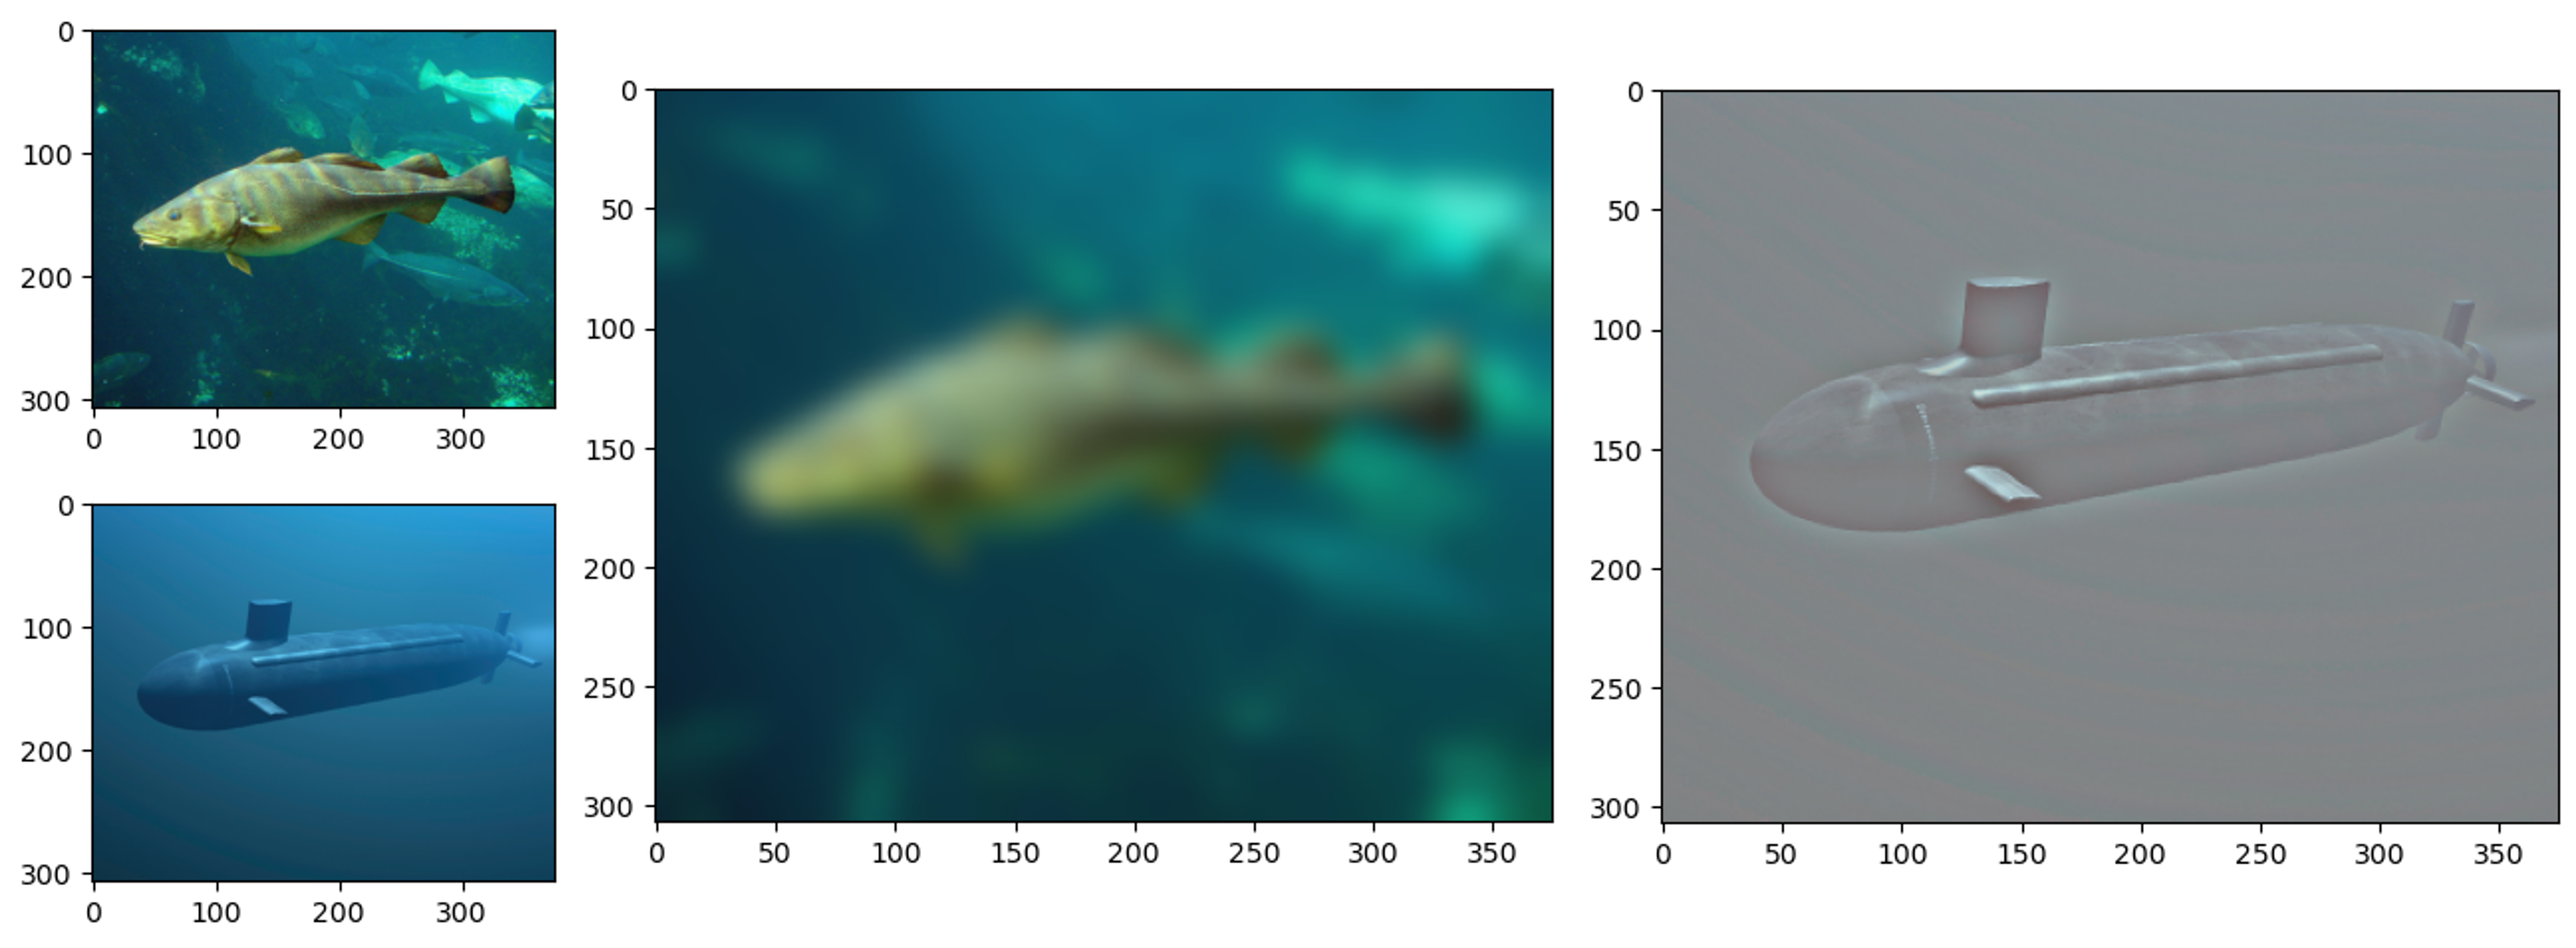
\includegraphics[width=0.7\linewidth]{image/图片4}
	\caption{鱼和鱼雷通过自定义的高低通滤波器的结果}
	\label{图3:}
\end{figure}



\begin{figure}
	\centering
	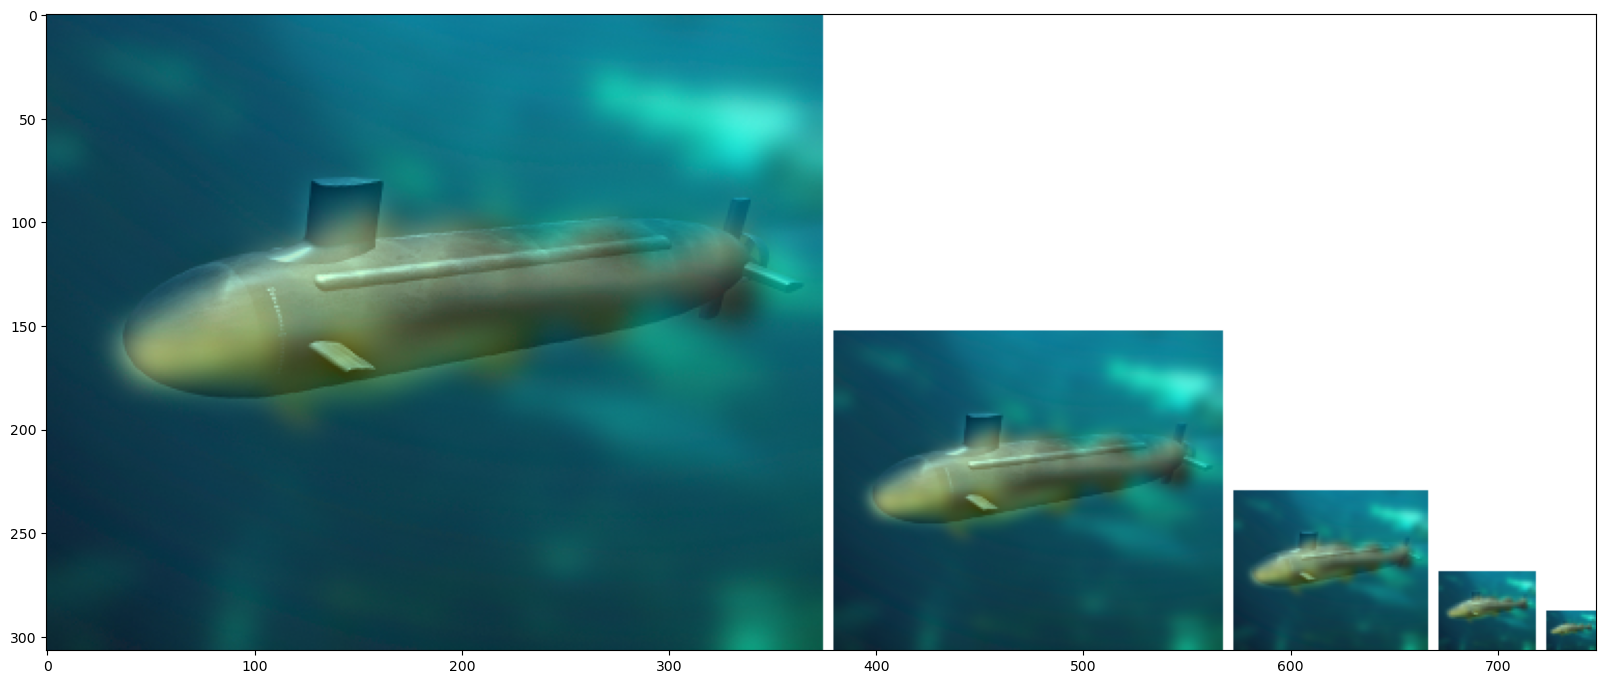
\includegraphics[width=0.7\linewidth]{image/hybrid}
	\caption{鱼和鱼雷融合图像}
	\label{图4:}
\end{figure}



\section{实验结论:}
从图2可以看到自行车的轮廓以不同方式显现出来,符合理论上我们对滤波器的认识;

从图3可以看到,当图片放大时,
相对我们在近距离观察时,
可以很明显地分辨它是鱼雷,但是当图片缩小时,
相对我们在远距离观察时,
可能会认为这是黄色的鱼,
这样的结果符合我们对高低通滤波器效果的认知。
这

以上结果说明我们的实验比较成功。

\section{总结及心得体会:}
尽管实验成功验证了核心原理并构建了基本框架,但也认识到当前实现作为生产级编译器前端存在诸多不足(如错误恢复的健壮性、符号表中信息的完整性、对复杂文法结构的处理能力、性能优化以及与现代编译器架构的差距等)。

总而言之,本次实验通过从零开始实现一个简单的编译器前端,不仅成功地将编译原理的理论知识转化为实际代码。 通过构建了一个可工作的简单demo,我加深了对词法分析、语法分析、作用域管理和符号表工作原理的理解。实验结果证明了所采用方法的有效性。

\section{对本实验过程及方法、手段的改进建议及展望:}
错误恢复机制 :本项目的词法分析器在遇到非法字符或错误时,会跳过当前行的剩余部分并返回错误。这是一种简单的恐慌模式错误恢复策略,即在检测到错误后,跳过一部分输入直到找到一个看似可以继续解析的同步点。可以设计更加用户友好的错误报告,比如“在 X 处期望得到 Y,但找到了 Z”,并给出可能的修正建议。还比如不仅仅跳到行尾,而是跳到更合适的同步词法单元,例如语句结束符 ;、块的开始/结束符号 (begin, end) 或文件末尾。这需要在文法中定义哪些词法单元可以作为同步点。

目前,对于变量声明的情况,无法维护其所属的过程名。在支持嵌套函数或过程的语言中,一个变量的完全限定名或用于查找作用域链的信息通常需要包含其所在的函数/过程信息。 在解析函数体或任何可能包含变量声明的块时,可以将当前正在解析的函数/过程的名称作为参数传递给其他方法,限于时间有限无法完成。

在文法中没有区分实参和形参,导致进一步语义分析可能出现了意料不到的错误。函数定义时的参数列表(形参)应该在函数体的局部作用域内进行声明,并且这些形参应该在函数体内部可见。这可能需要修改文法来明确区分函数定义和函数调用,并为函数定义引入形参列表的文法规则,例如 <形参列表> → <变量> { , <变量> } | ε

我们只对文件流进行了简化实现,在prep.rs 中的文件不足可能在于错误处理比较简单,以及没有考虑字符编码问题。lex.rs 和 parse.rs 中的文件错误输出每次都会新建并覆盖文件,没有追加功能。而且错误应该输出到标准错误流而不是标准输出,这在命令行工具中是更好的实践。应该采用更安全的IO方式;

lex.rs 中的 current_token 方法是手写的状态转换逻辑,模拟了有限自动机。
手写 DFA 对于简单文法是可行的,但对于复杂语言,状态和转换会变得非常多且难以管理,容易出错。之后可以尝试手动实现一个表驱动的 DFA,根据当前状态和输入字符查找下一个状态。

输入优化:Lexer 在 getchar 中使用下标索引的来获取字符。这种方式在 pos 较大时效率较低,因为它需要从字符串的开头开始遍历字符直到 pos 位置.更好的方式是使用 
缓冲读取,对于非常大的文件,可以考虑实现或使用带缓冲的文件读取,而不是一次性将整个文件读入内存。


\vspace{4cm}
\begin{flushright}
\begin{tabular}{lc}
\sihao{\hei{报告评分:}}& \sihao{\song{~~~~~~}}\\
\sihao{\hei{指导教师签字:}}& \sihao{\song{~~~~~~}}\\
\end{tabular}
\end{flushright}

\newpage

\begin{appendix}
\section{核心代码}

如代码 1 所示。

\begin{lstlisting}[caption={student.py}, label={lst:code-example}, captionpos=t, language=python]
    # Project Image Filtering and Hybrid Images Stencil Code
    # Based on previous and current work
    # by James Hays for CSCI 1430 @ Brown and
    # CS 4495/6476 @ Georgia Tech
    import numpy as np
    from numpy import pi, exp, sqrt
    from skimage import io, img_as_ubyte, img_as_float32
    from skimage.transform import rescale
    import math
    
    def my_imfilter(image, filter):
      """
      Your function should meet the requirements laid out on the project webpage.
      Apply a filter to an image. Return the filtered image.
      Inputs:
      - image -> numpy nd-array of dim (m, n, c)
      - filter -> numpy nd-array of odd dim (k, l)
      Returns
      - filtered_image -> numpy nd-array of dim (m, n, c)
      Errors if:
      - filter has any even dimension -> raise an Exception with a suitable error message.
      """

      image_height, image_width = image.shape[:2]
      filter_height, filter_width = filter.shape
      num_channels = 1 if image.ndim == 2 else image.shape[2]
    
      # Calculate padding amounts
      pad_height = filter_height // 2
      pad_width = filter_width // 2
      padded_image = np.pad(image, ((pad_height, pad_height), (pad_width, pad_width), (0, 0) if num_channels > 1 else (0, 0)), mode='reflect')
    
      # filter process: convolution
      filtered_image = np.zeros_like(image)
      flipped_filter = np.flip(filter, axis=(0, 1))
      for c in range(num_channels):
          for i in range(image_height):
              for j in range(image_width):
                  image_patch = padded_image[i:i+filter_height, j:j+filter_width, c] if num_channels > 1 else padded_image[i:i+filter_height, j:j+filter_width]
                  
                  filtered_image[i, j, c] = np.sum(image_patch * flipped_filter) if num_channels > 1 else np.sum(image_patch * flipped_filter)
      return filtered_image
    
    
    def gen_hybrid_image(image1, image2, cutoff_frequency):
      """
       Inputs:
       - image1 -> The image from which to take the low frequencies.
       - image2 -> The image from which to take the high frequencies.
       - cutoff_frequency -> The standard deviation, in pixels, of the Gaussian
                             blur that will remove high frequencies.
    
       Task:
       - Use my_imfilter to create 'low_frequencies' and 'high_frequencies'.
       - Combine them to create 'hybrid_image'.
      """
    
      assert image1.shape[0] == image2.shape[0]
      assert image1.shape[1] == image2.shape[1]
      assert image1.shape[2] == image2.shape[2]
    
      # Steps:
      # (1) Remove the high frequencies from image1 by blurring it. The amount of
      #     blur that works best will vary with different image pairs
      # generate a 1x(2k+1) gaussian kernel with mean=0 and sigma = s, see https://stackoverflow.com/questions/17190649/how-to-obtain-a-gaussian-filter-in-python
      s, k = cutoff_frequency, int(cutoff_frequency*2)
      probs = np.asarray([exp(-z*z/(2*s*s))/sqrt(2*pi*s*s) for z in range(-k,k+1)], dtype=np.float32)
      kernel = np.outer(probs, probs)
      
      # Your code here:
      # low_frequencies = None # Replace with your implementation
      low_frequencies = my_imfilter(image1, kernel)
    
      # (2) Remove the low frequencies from image2. The easiest way to do this is to
      #     subtract a blurred version of image2 from the original version of image2.
      #     This will give you an image centered at zero with negative values.
      # Your code here #
      # high_frequencies = None # Replace with your implementation
      image2_low_frequencies = my_imfilter(image2, kernel)
      high_frequencies = image2 - image2_low_frequencies
    
      # (3) Combine the high frequencies and low frequencies
      # Your code here #
      # hybrid_image = None
      hybrid_image = low_frequencies + high_frequencies
    
      # (4) At this point, you need to be aware that values larger than 1.0
      # or less than 0.0 may cause issues in the functions in Python for saving
      # images to disk. These are called in proj1_part2 after the call to 
      # gen_hybrid_image().
      # One option is to clip (also called clamp) all values below 0.0 to 0.0, 
      # and all values larger than 1.0 to 1.0.
      hybrid_image = np.clip(hybrid_image, 0, 1)

      return low_frequencies, high_frequencies, hybrid_image
    
    def vis_hybrid_image(hybrid_image):
      """
      Visualize a hybrid image by progressively downsampling the image and
      concatenating all of the images together.
      """
      scales = 5
      scale_factor = [0.5, 0.5, 1]
      padding = 5
      original_height = hybrid_image.shape[0]
      num_colors = 1 if hybrid_image.ndim == 2 else 3
    
      output = np.copy(hybrid_image)
      cur_image = np.copy(hybrid_image)
      for scale in range(2, scales+1):
        # add padding
        output = np.hstack((output, np.ones((original_height, padding, num_colors),
                                            dtype=np.float32)))
        # downsample image
        cur_image = rescale(cur_image, scale_factor, mode='reflect')
        # pad the top to append to the output
        pad = np.ones((original_height-cur_image.shape[0], cur_image.shape[1],
                       num_colors), dtype=np.float32)
        tmp = np.vstack((pad, cur_image))
        output = np.hstack((output, tmp))
      return output
    
    def load_image(path):
      return img_as_float32(io.imread(path))
    
    def save_image(path, im):
      return io.imsave(path, img_as_ubyte(im.copy()))
    
\end{lstlisting}
\end{appendix}

\end{document}
